\documentclass[default]{beamer}
\setbeamertemplate{navigation symbols}{}

\usetheme{CambridgeUS}
\useoutertheme{infolines}
%\usecolortheme{crane}

\usepackage[utf8]{inputenc}					% Выбор языка и кодировки
\usepackage{tikz}
\usepackage{animate}
\usepackage{fp}

\usetikzlibrary{calc,patterns,backgrounds}

\graphicspath{{../../images/}} 			% Пути к изображениям

\makeatletter
\setbeamertemplate{footline}
{
	\leavevmode%
	\hbox{%
		\begin{beamercolorbox}[wd=.333333\paperwidth,ht=2.25ex,dp=1ex,center]{author
				in head/foot}%
			\usebeamerfont{author in
				head/foot}\insertshortauthor~~\beamer@ifempty{\insertshortinstitute}{}{(\insertshortinstitute)}
		\end{beamercolorbox}%
		\begin{beamercolorbox}[wd=.333333\paperwidth,ht=2.25ex,dp=1ex,center]{title in
				head/foot}%
			\usebeamerfont{title in head/foot}\insertshorttitle
		\end{beamercolorbox}%
		\begin{beamercolorbox}[wd=.333333\paperwidth,ht=2.25ex,dp=1ex,right]{date in
				head/foot}%
			\usebeamerfont{date in head/foot}\insertshortdate{}\hspace*{2em}
			\insertframenumber{}\hspace*{2ex} 
		\end{beamercolorbox}
	}%
	\vskip0pt%
}

\newcommand{\blockp}[3]{
	\node[draw, rectangle, pattern = #3, minimum width = #1, minimum height = #2] 
}

\newcommand{\situation}[4]{
	\begin{tikzpicture}
		\blockp{150}{20}{crosshatch} at (0,0) {};
		\blockp{150}{20}{crosshatch} at (10,0) {};
		
		\blockp{20}{40}{crosshatch} at (1.5,-1.5) {};
		\blockp{20}{40}{crosshatch} at (2.5,-3) {};
		
		\blockp{40}{20}{crosshatch} at (4.7,-4.5) {};
		\blockp{20}{15}{north west lines} at (6.5,-2) {};				
		
		\blockp{20}{40}{crosshatch} at (6,-3.1) {};
		\blockp{20}{30}{crosshatch} at (7,-1) {};
		
		\node[draw, circle, dotted, very thick, minimum width = 50, text = black] (goal) at (5, -1) {$G$};
		\node[draw, gray, circle, dotted, very thick, minimum width = 30, text = black] (confl_2) at (6.5, -2) {};				
		\node at (7.5, -2) {$obs_2$};

		\node[draw, gray, fill = gray, circle, very thick, minimum width = 20] (obj_1) at (#1, #2) {};
		\node at (4, -6.8) {$A_1$};						
		\node[draw, gray, fill = gray, circle, very thick, minimum width = 20] (obj_2) at (#3, #4) {};
		\node at (10, -3.3) {$A_2$};

		\draw[->, very thick, gray] (obj_2) edge (goal);				
		\blockp{20}{20}{north west lines} at (3.4,-4.5) {};				
		\node[draw, gray, circle, dotted, very thick, minimum width = 40, text = black] (confl_1) at (3.3, -4.3) {};
		\node at (2.2, -4.2) {$obs_1$};								


		\draw[->, very thick, dotted, gray] (obj_1) edge [bend left, out = 80, in = 150] (goal);
	\end{tikzpicture}
}

\begin{document}
	
	\title[Behavior and path planning]{Behavior and path planning for the coalition of cognitive robots in smart relocation tasks}
	\author[Panov, Yakovlev]{Aleksandr Panov, Konstantin Yakovlev}
	
	\institute[FRC CSC]{Institute for Systems Analysis of Federal Research Center ``Computer Science and Control''}
	\date{December 18, 2015} 
	
	\begin{frame}
		\titlepage
	\end{frame}
	
	\begin{frame}
		\frametitle{STRL architecture}
		
		\begin{figure}
			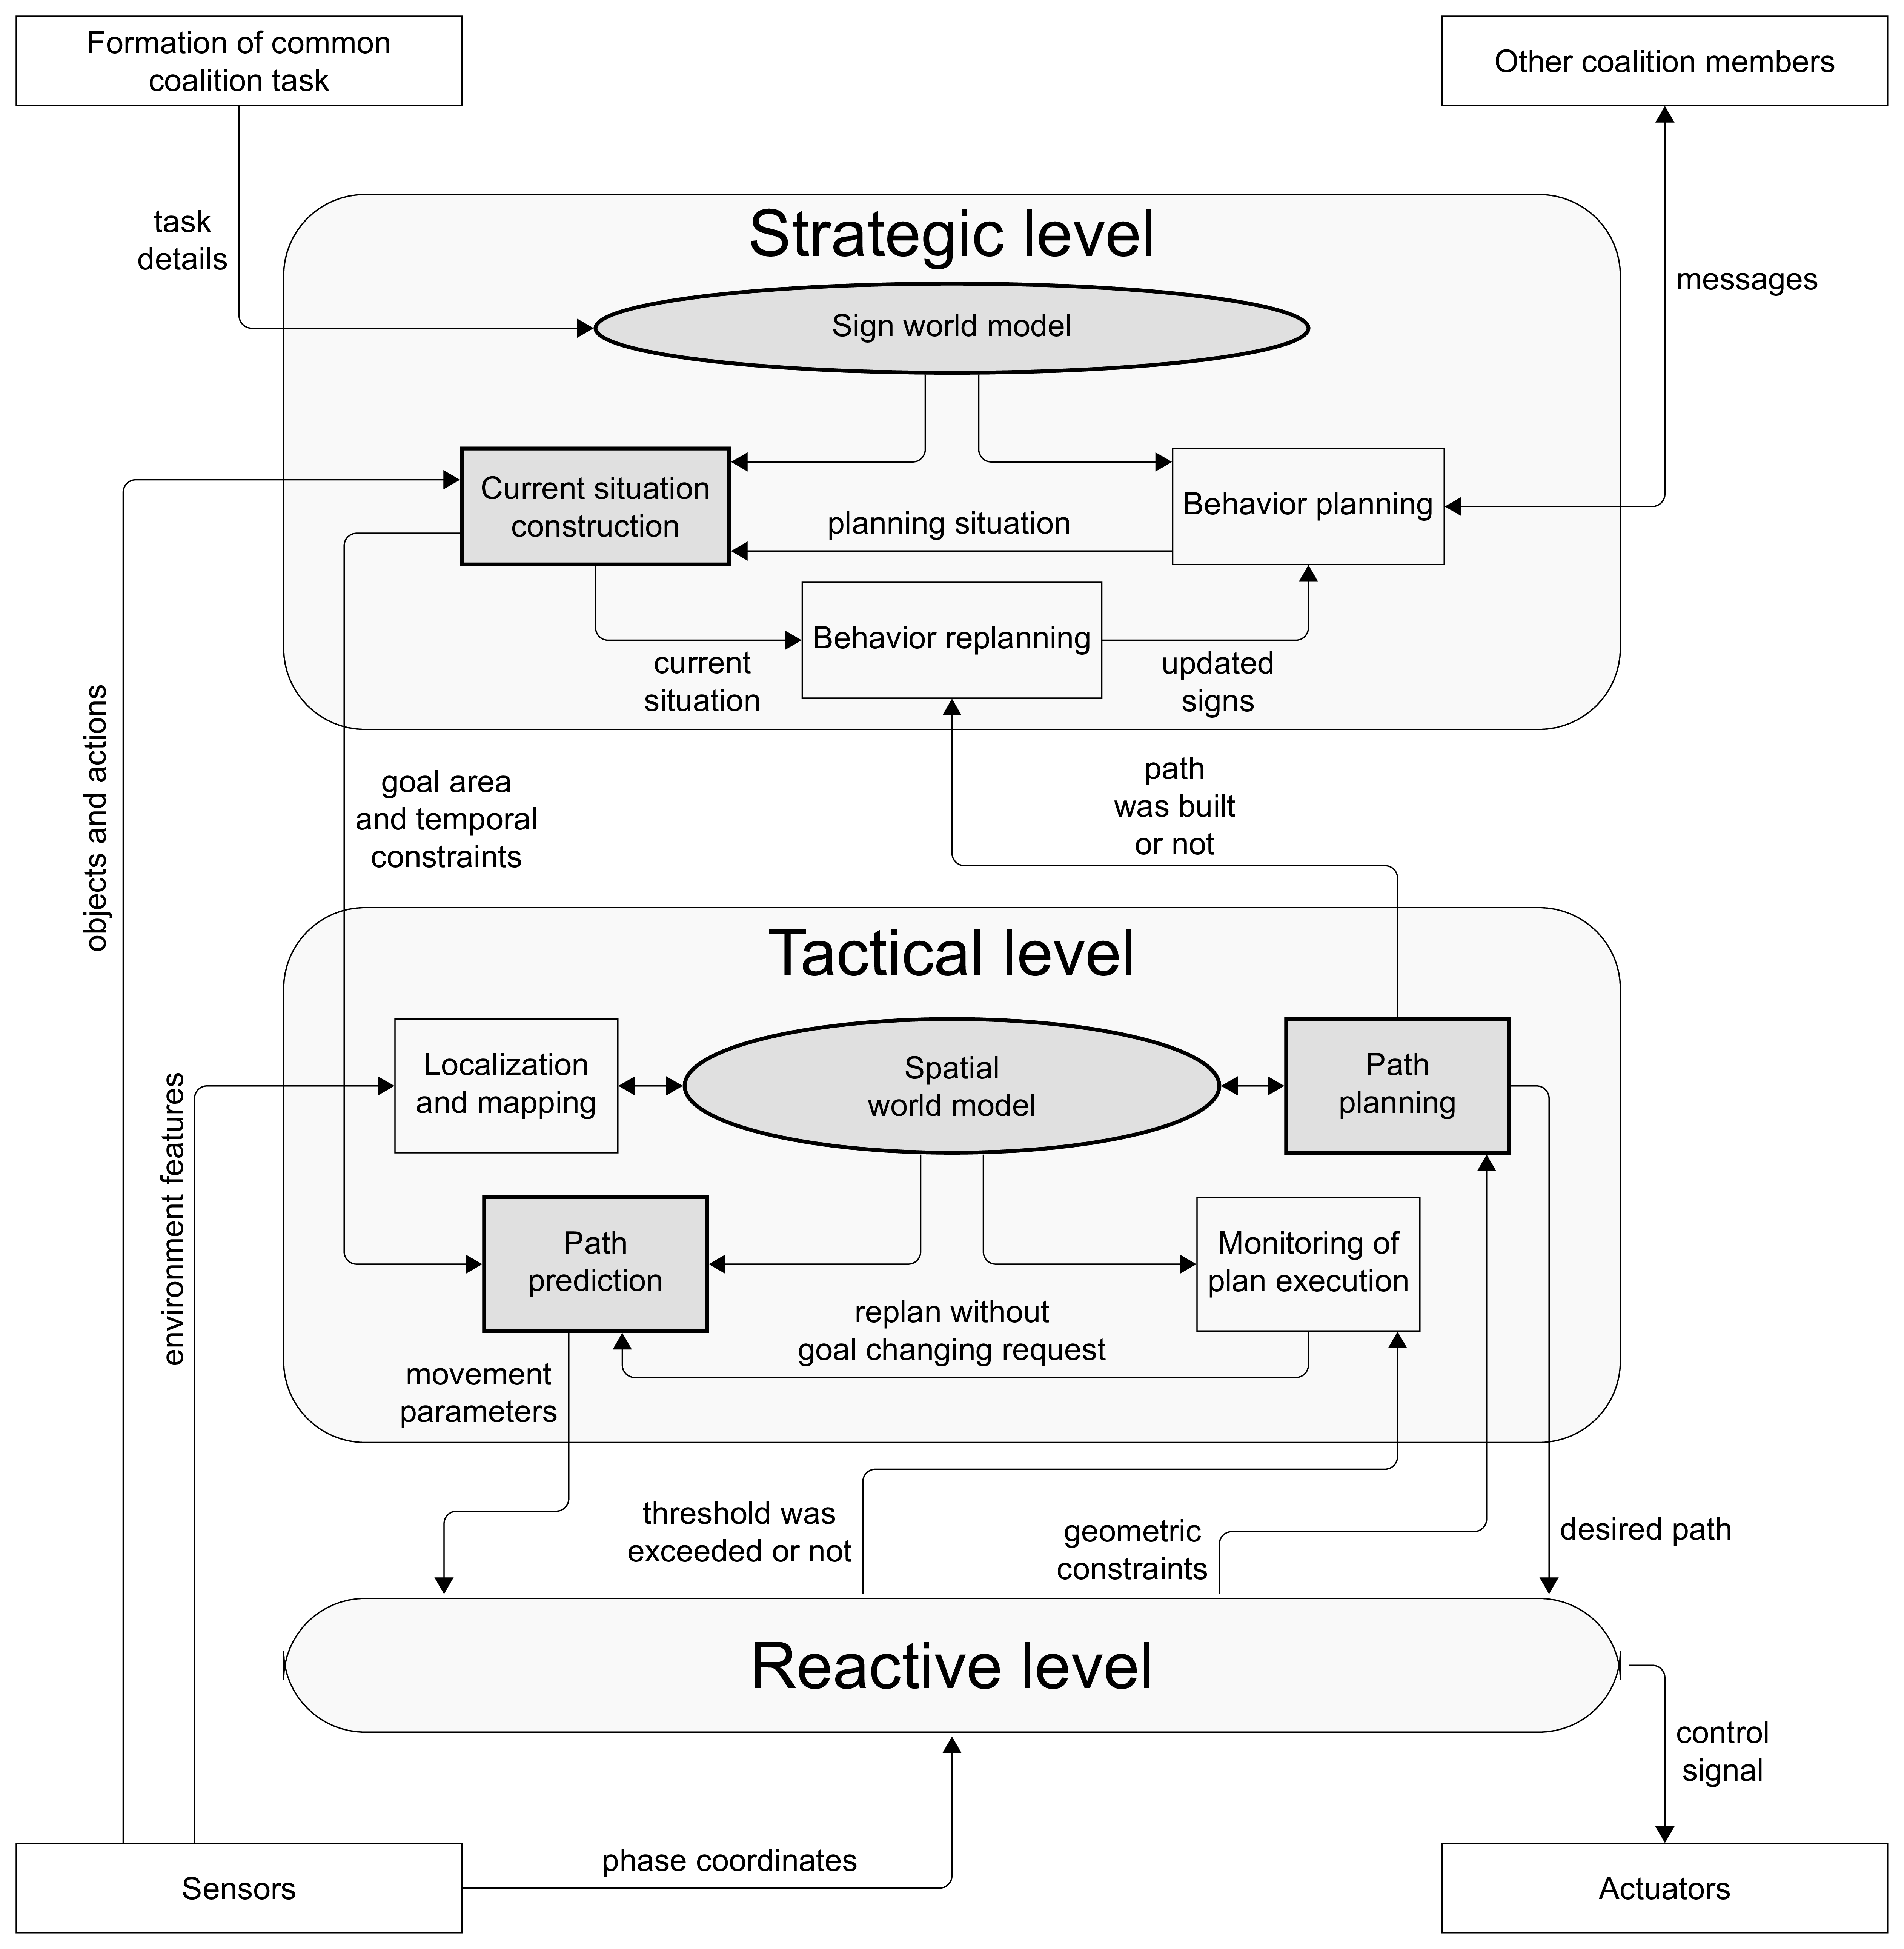
\includegraphics[width=0.6\textwidth]{strl/strl_rita_eng.png}
		\end{figure}
	\end{frame}
		
	\begin{frame}
		\frametitle{Movie}
		\begin{center}
			\scalebox{0.7}{
				\animategraphics{12}{slides_colored}{}{}			
			}
		\end{center}
	\end{frame}		

	\begin{frame}
		\centering
		\Huge
		Thank you for attention!
		\normalsize
		\par\bigskip
		\par\bigskip
		FRC CSC RAS, Lab. ``Dynamic Intelligent Systems'', pan@isa.ru
	\end{frame}
									
	%	\begin{frame}
	%		\frametitle{Цели курса}
	%		
	%		\begin{itemize}
	%			\item
	%		\end{itemize}
	%	\end{frame}
	
\end{document}
	
	
